\documentclass{standalone}
\usepackage{tikz}

\begin{document}

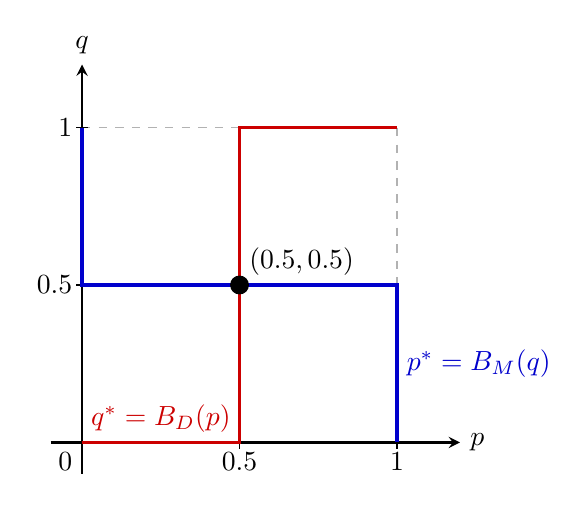
\begin{tikzpicture}[scale=4, >=stealth]
    % Axes
    \draw[->, thick] (-0.1, 0) -- (1.2, 0) node[right] {$p$};
    \draw[->, thick] (0, -0.1) -- (0, 1.2) node[above] {$q$};

    % Unit square bounding box (dashed)
    \draw[dashed, gray!60] (0, 1) -- (1, 1) -- (1, 0);

    % Axis labels/ticks
    \node[below left] at (0, 0) {$0$};
    \node[below] at (0.5, 0) {$0.5$};
    \node[below] at (1, 0) {$1$};
    \node[left] at (0, 0.5) {$0.5$};
    \node[left] at (0, 1) {$1$};

    % Tick marks
    \draw (0.5, 0.02) -- (0.5, -0.02);
    \draw (1, 0.02) -- (1, -0.02);
    \draw (0.02, 0.5) -- (-0.02, 0.5);
    \draw (0.02, 1) -- (-0.02, 1);

    % Best response B_D(p) - Red Line
    % For p < 0.5, q = 0
    % For p = 0.5, q in [0, 1]
    % For p > 0.5, q = 1
    \draw[very thick, red!80!black] (0, 0) -- (0.5, 0) -- (0.5, 1) -- (1, 1);

    % Best response B_M(q) - Blue Line
    % For q < 0.5, p = 1
    % For q = 0.5, p in [0, 1]
    % For q > 0.5, p = 0
    \draw[very thick, blue!80!black] (1, 0) -- (1, 0.5) -- (0, 0.5) -- (0, 1);

    % Nash Equilibrium Point
    \filldraw[black] (0.5, 0.5) circle (0.8pt);
    \node[above right] at (0.5, 0.5) {$(0.5, 0.5)$};

    % Legend / Curve Labels
    \node[blue!80!black, right] at (1, 0.25) {$p^* = B_M(q)$};
    \node[red!80!black, above] at (0.25, 0) {$q^* = B_D(p)$};

\end{tikzpicture}

\end{document}
